\documentclass[11pt,a4paper]{article}
\usepackage[utf8]{inputenc}
\usepackage{amsmath}
\usepackage{amsfonts}
\usepackage{amssymb}
\usepackage{graphicx}
\usepackage{mathtools}
\usepackage[backend=bibtex,style=verbose-ibid]{biblatex}
\addbibresource{citations.bib}


\usepackage{listings}
\usepackage{color}
\definecolor{dkgreen}{rgb}{0,0.6,0}
\definecolor{gray}{rgb}{0.5,0.5,0.5}
\definecolor{mauve}{rgb}{0.58,0,0.82}

\lstset{frame=tb,
  language=Python,
  aboveskip=3mm,
  belowskip=3mm,
  showstringspaces=false,
  columns=flexible,
  basicstyle={\small\ttfamily},
  numbers=none,
  numberstyle=\tiny\color{gray},
  keywordstyle=\color{blue},
  commentstyle=\color{dkgreen},
  stringstyle=\color{mauve},
  breaklines=true,
  breakatwhitespace=true,
  tabsize=3
}


\newcommand{\inv}{^{\raisebox{.2ex}{$\scriptscriptstyle-1$}}}
\newcommand{\qed}{\hfill $\blacksquare$}
\newcommand{\reals}{\mathbb{R}}
\newcommand{\complexes}{\mathbb{C}}
\newcommand{\field}{\mathbb{F}}
\author{Jacob Bruner}
\title{IB Extended Essay}
\date{\today}

\begin{document}
\maketitle
\tableofcontents

\pagebreak

\iffalse
############
heres an example of a code block
\begin{lstlisting}
        def intervalValues(z, n):
            return output # return the sequence of values
\end{lstlisting}

heres an example of an image
\begin{figure}[h]
\begin{center}
\includegraphics[scale=.37]{onefifteen} 
\caption{Sequences Generated by n = 1-15 on Argand Diagram}
\end{center}
\end{figure}
############
\fi

\section{Introduction and Aim}
\subsection{Motivating Problem}
It's undeniable that our modern-day world is reliant on cryptography. Every time a phone sends a text, a browser connects to a server, an email gets sent off, a monetary transaction is made, and much much more, our devices are, unbeknownst to us, performing many hundreds of math operations to ensure our data are 'encrypted.' But what does 'encryption' mean? Let's introduce some definitions. ‘Encryption’ is the process of disguising a message to be, loosely speaking, hidden to all but the intended recipient. This is the process of converting a ‘plaintext’ message into a jumbled ‘ciphertext’, which can be readily shared without risk of the sensitive message leaking. Converting a plaintext message (typically a string/list of characters) into a ciphertext is known as an ‘enciphering’ or ‘encrypting’ transformation. Likewise the reverse operation of recovering the plaintext message from a ciphertext is known as the \textit{deciphering transformation.}\autocite[54]{koblitz} If we denote the plain and cyphertext $\mathcal{P}$ and $\mathcal{C}$ respectively and the enciphering map $f$ and its inverse $f\inv$ we obtain the following diagram:

$$ \mathcal{P} \overset{f}\longrightarrow \mathcal{C} \overset{f\inv}\longrightarrow \mathcal{P} $$

The most common formulation for this kind of cryptosystem would be that the two transacting parties agree upon the parameters for the map $f$ in secret beforehand. Common examples include the 'Caeser Cipher' (supposedly invented by \textit{the} Julius Caeser), where $f$ is a shift operation that maps each letter to a new one a number of places ahead. We start encoding each letter as a number from 0, which is A, to 25, which is Z. Of course this depends on what alphabet one uses, if one chooses to include spaces etc. We can represent the operation that takes a letter and maps it $n$ places ahead with addition. Importantly, this operation must 'wrap around' back to zero if you try to exceed 'z' in the alphabet. This process, known as \textit{'modular arithmetic'}, is like circling a clock, where after reaching twelve, the hour hand wrap back around to 1, but we start from 0 instead of 1. So, in our case, shifting 'z' by 3 letters looks like so: $25 + 1 \bmod 26 \equiv 0$, which reads "25 plus 1 \textit{is congruent to} 0 \textit{modulo} (or \textit{mod}) 26". With this in mind, we obtain for each letter $p \in \mathcal{P}$:

\[
f(p) = p + n \bmod 26
\]

% I could maybe talk about affine cryptosystems here if I need more words.
% I could also show the linear algebra point of view

Representing a shifting of each letter in the plaintext by $n$ places in the alphabet. Now clearly this isn't a very sophisticated cryptographic scheme. For instance, performing a frequency analysis and comparing the most commonly occurring letters to that of the English alphabet can easily break these sorts of schemes, known as 'substitution ciphers.' Modern schemes typically employ more resistant techniques such that changing one letter of plaintext often yields a completely different ciphertext.
  For instance, AES encryption, part of the modern web standard, is an example of a block substitution cypher. At a high level, it combines techniques similar to our Caesar Cipher with certain affine transformations (which can be thought of as an additional scaling action in combination with our translation) performed on blocks of plaintext. It's certainly more complicated than that, but essentially boils down to our system plus some bells and whistles to make it resistant to cryptanalysis, like permutations, combinations, text look-up-tables and more. In general, this type of encryption where there's a predetermined shared secret is well-studied, often bearing the name 'symmetric-key encryption,' to emphasize that the private keys are known beforehand. For instance, Claude Shannon (often called the father of cryptography) mathematically proved that the 'one-time-pad' encryption technique was unbreakable. His findings showed that if a random-generated key is at least as long as the plaintext, performing modular addition (i.e., wrapping around so as to not exceed the alphabet) on each letter by the private key yields a ciphertext that is uncrackable.\autocite{claude} Although modern systems seek smaller key sizes for performance reasons, this worst-case scenario should demonstrate the strength of symmetric-key algorithms in general. The 'one-time-pad' gets its name from its use in WWII when the KGB would distribute palm-sized pads with these one-time-keys and a table to ease in conversion. Such pads were often made of flammable materials to be burned with no trace.\autocite{lewand} 
  
\begin{figure}[h]
\begin{center}
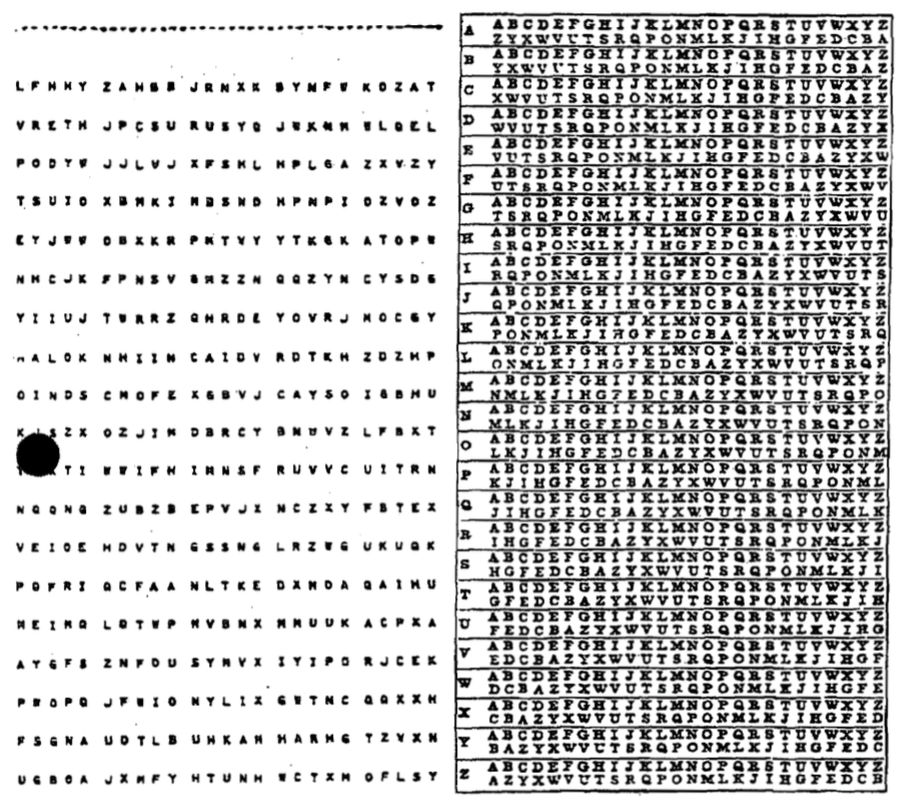
\includegraphics[scale=.25]{images/diana} 
\caption{Format of a one-time-pad used by the NSA\autocite{diana}}
\end{center}
\end{figure}
  

\subsection{The 'Public-Key' Paradox}


\section{What is 'Public-Key' Cryptography}
The first protocol developed to address this motivating problem was RSA encryption. Leveraging intuitive properties of numbers, RSA establishes our idea of ‘one-way operations’ using simple multiplication of large, highly prime (minimal divisors), numbers. 

\section{How can we formalize this: An Introduction to Groups}
Group theory provides us a way to generalize certain, often intuitive, properties of number systems, by using axiomatic structure to classify groups ‘up to isomorphism’ and to prove various properties about their structures. A ‘Group’ boils down to a set, infinite or finite, and an operation that takes two elements and maps it to another while maintaining some structure. It’s common to think that this structure is too vague, or broad, but, in fact, it’s enough to prove sweeping conjectures and determine non-trivial properties, thereby making itself a staple of modern mathematics.


\section{Group Law on an Elliptic Curve}
While the elliptic curve group admits an intuitive geometric description, it's important that our algebraic description satisfies the group axioms.  $ E(\field_{q} )$ 
\autocite[10]{koblitz}

\newpage 

\printbibliography

\end{document}